\documentclass[../manuscript.tex]{subfiles}

\section{Материалы и методы}
Данный метод разработан для задачи поиска малых молекул, способных вызвать нужные изменения в фенотипе клетки. Поскольку для достижения больших изменений не достаточно одного соединения, в этой задаче актуальна проблема поиска синергетических комбинаций химических соединений. Наш подход позволяет оценить уровень синергии каждой пары соединений и, соответственно, приоритезировать список пар малых молекул по уровню синергии. В его основе лежит работа с экспрессионными сигнатурами и генными сетями.

Экспрессионные сигнатуры позволяют охарактеризовать разницу между двумя состояниями клеток. Мы используем базу данных \href{https://amp.pharm.mssm.edu/l1000fwd/}{L1000FWD} \cite{10.1093/bioinformatics/bty060}, которая содержит 42809 сигнатур, возмущенных малыми молекулами на разных клеточных линиях. Для каждой малой молекулы из рассматриваемого набора мы находим индуцированные ею сигнатуры в базе L1000FWD. Таким образом, для конкретного набора малых молекул создается набор сигнатур из L1000FWD. Чтобы найти пары малых молекул, которые вызовут желаемые изменения в экспрессии генов, мы будем сравнивать соответствующие пары сигнатур с желаемой сигнатурой. На основе этого сравнения будет рассчитан уровень синергии малых молекул.


Метод можно использовать в 2 режимах:
\begin{itemize}
    \item "прямой"\ - позволяет искать синергетические комбинации малых молекул для индуцирования нужных изменений в фенотипе клетки 
    \item "обратный"\ - позволяет искать синергетические комбинации малых молекул для обращения изменений в фенотипе клетки
\end{itemize}



Рассмотрим метод подробнее. В нем можно выделить 2 основных этапа:
\begin{itemize}
    \item создание экспрессионной сигнатуры запроса
    \item вычисление уровня синергии пары малых молекул
\end{itemize}

\subsection{Создание экспрессионной сигнатуры запроса}
Для описания желаемых изменений в фенотипе клетки используется экспрессионная сигнатура. На основе данных RNA-seq для начального и конечного состояния клетки проводится анализ дифференциальной экспрессии с использованием пакета edgeR, затем отбираются гены по значениям logFC и p-уровню значимости. Полученная генная сигнатура далее будет использована для сравнения. 
При сравнении сигнатур мы хотим учитывать биологическую значимость генов в  данном контексте, то есть нас интересуют сигнатуры, которые схожи по наиболее значимым генам. Таким образом, одна из основных целей этой работы - создать метод, который оценивает биологическую значимость гена в данном контексте, и при пересечении сигнатур гены будет иметь вес в соответствии с их биологической значимостью.


Чтобы определить важность генов в сигнатуре запроса, мы строим 2 генные сети, одна для генов с повышенной экспрессией, вторая для генов с пониженной экспрессией. При построении сети информация о взаимодействиях берется из базы данных \href{https://string-db.org/cgi/input?sessionId=bLkChLc5rf5a&input_page_show_search=on}{STRING} \cite{10.1093/nar/gky1131}, которая включает в себя как известные, так и предсказанные взаимодействия. Эти взаимодействия включают в себя прямые и косвенные связи; они создаются на основе вычислительного прогнозирования, переноса знаний между организмами, взаимодействий, агрегированных из других (первичных) баз данных. Пять основных источников базы данных STRING: предсказания в контексте генома, высокопроизводительные лабораторные эксперименты, коэкспрессия, автоматизированный интеллектуальный анализ текстов, прежние сведения в базах данных. К сожалению, API запрос в базу данных STRING позволяет узнать о взаимодействиях генов между собой для наборов, содержащих не более 2000 генов, поэтому сети были ограничены 2000 узлами. Для большинства рассмотренных сигнатур количество генов с повышенной или пониженной экспрессией в сигнатуре больше 2000. Поэтому производился отбор 2000 генов с большими значениями модуля logFC, про которых есть сведения в базе STRING.

Поскольку была показана связь между биологической значимостью белка и топологическими метриками, такими как betweenness и closeness \cite{hahn2005comparative}, \cite{joy2005high}, то в данном подходе уровень значимости рассчитывается по метрикам центральности, среди которых есть betweenness (Btw) и closeness (Cln). 


Betweenness (Btw) для вершины $\upsilon$ определяется следующим образом:
\begin{equation}
    Btw(\upsilon)=\sum_{\text{\makecell{$s \neq \upsilon \neq t \in V$\\$s\neq t$}}}^{}{\frac{\sigma_{st}(\upsilon)}{\sigma_{st}}}\text{,}
    \label{Btw}
\end{equation}
где $\sigma_{st}$ - количество кратчайших путей от вершины s до вершины t, $\sigma_{st}(\upsilon)$ - количество кратчайших путей от вершины s до вершины t через вершину $\upsilon$.


Closeness (Cln) для вершины i определяется следующим образом:
\begin{equation}
    {Cln}_i=\frac{1}{\sum_{j}^{}{d_{ij}}}\text{,}
    \label{(Cln}
\end{equation}
где $d_{ij}$ - расстояние от вершины i до j. Если нет пути между этими вершинами, то расстояние считается равным 0.


Также при расчете уровень значимости гена были включены другие топологические метрики: pagerank (Prk), eigenvector centrality (Egv), Katz centrality (Ktz), eigentrust (Egt).


Pagerank (Prk) для вершины $\upsilon$ определяется следующим образом:
\begin{equation}
    {Prk}(\upsilon) = \frac{1-d}{N} + d \sum_{u \in \Gamma^{-}(\upsilon)}^{}{\fraq{Prk(u)}{d^{+}(u)}}\text{,}
    \label{Prk}
\end{equation}
где $\Gamma^{-}(\upsilon)$ - набор соседних вершин, которые ссылаются на вершину $\upsilon$, $d^{+}(u)$ - число выходящих ребер из вершины u, d - коэффициент затухания. 


Eigenvector centrality(Egv) определяется как собственный вектор X матрицы смежности для наибольшего собственного значения, то есть является решением:
\begin{equation}
    \textbf{Ax} = \lambda \textbf{x}\text{,}
    \label{Egv}
\end{equation}
где \textbf{A} - матрица смежности, $\lambda$ - наибольшее собственное значение.


Katz centrality (Ktz) определяется как решение неоднородной линейной системы:
\begin{equation}
      \textbf{x} = \alpha \textbf{Ax} + \textbf{1}\text{,}
    \label{Ktz}
\end{equation}
где \textbf{A} - матрица смежности, $\alpha $ - коэффициент ослабления.

Eigentrust (Egt) определяется следующим образом:
\begin{equation}
      \textbf{Egt} = \lim_{n\to \infty}{{({\textbf{C}}^T)}^n}\textbf{c}\text{,}
    \label{Egt}
\end{equation}
где $c_i = \frac{1}{|V|}$, элементы матрицы \textbf{С} представляют собой нормализованные значения доверия:
\begin{equation}
     c_{ij} = \frac{max(s_{ij},0)}{\sum_{j}^{}{max(s_{ij},0)}}
    \label{Egt}
\end{equation}
В качестве $s_{ij}$ использовались значения достоверности предсказания взаимодействия генов из базы данных STRING.

Все выше указанные метрики реализованы в пакете Graph-tool. Все топологические метрики и значения logFC, взятые по модулю, были нормализованы так, чтобы их значения были распределены от 0 до 1.


Уровень биологической значимости гена на основе топологических метрик центральности и значения модуля logFC вычислялся следующим образом:


 $inf\_score = (a_1 \cdot |log{FC}| + 1) \cdot (a_2 \cdot \textrm{Prk} + 1)\cdot(a_3 \cdot \textrm{Btw} + 1 )\\
\cdot(a_4 \cdot \textrm{Egv} + 1) \cdot (a_5 \cdot \textrm{Cln} + 1) \cdot (a_6 \cdot \textrm{Ktz} + 1) \cdot (a_7 \cdot \textrm{Egt} + 1) \text{,} $


где $a_1, a_2 \text{...} a_7 $- числовые коэффициенты. Они были подобраны на основании масштабной валидации на базе данных CFM \cite{cfm}, которая будет подробно освещена дальше.


Если для гена не были рассчитаны топологические метрики, то уровень значимости рассчитывается только по значению logFC:
\begin{equation}\label{formula1}
inf\_score = (a_1 \cdot \log{FC} + 1)
\end{equation}
Ниже представлена схема основных этапов создания сигнатуры запроса.
\begin{figure}[H]
\center{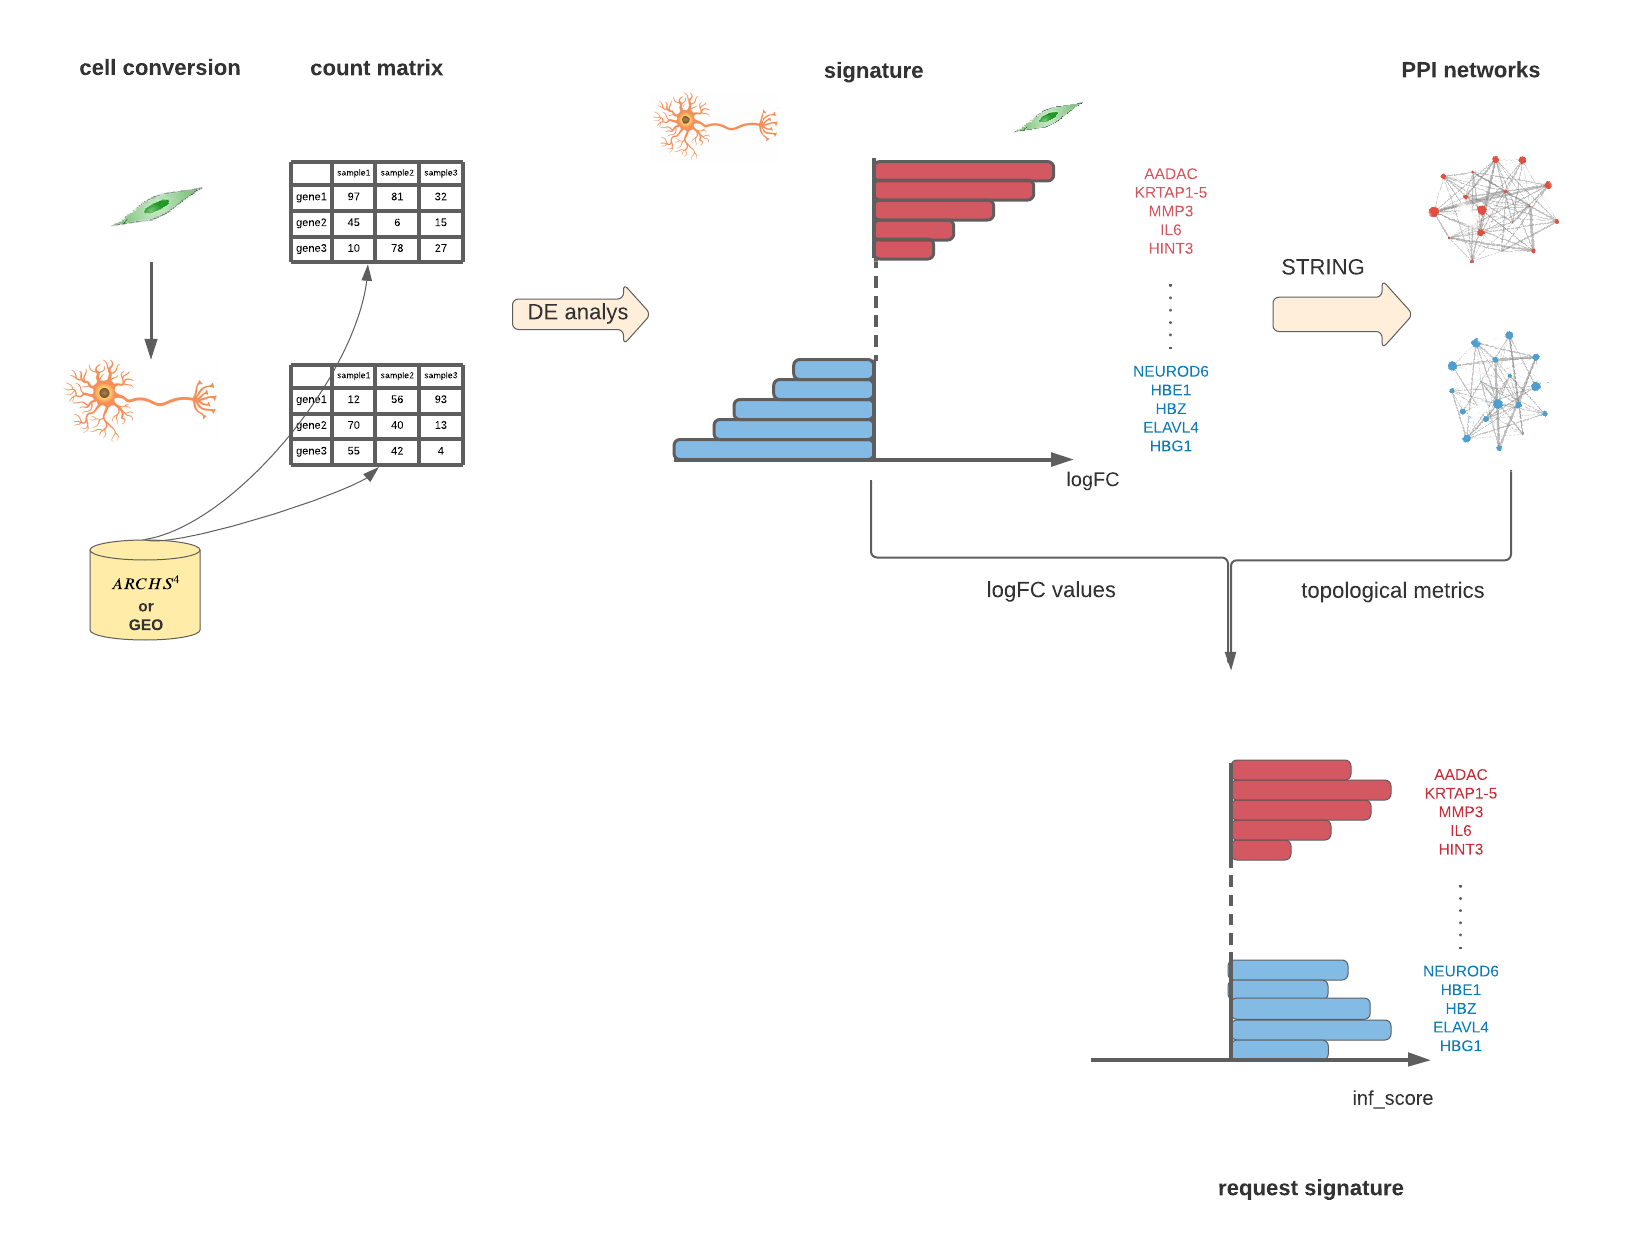
\includegraphics[width=0.7\linewidth]{images/signature.png}}
\caption{создание экспрессионной сигнатуры запроса}
\end{figure}

 
\subsection{Вычисление уровня синергии}
Для каждой пары сигнатур из вычисляется уровень синергии. Он считается 2 способами:
\begin{itemize}
    \item Вычисление уровня синергии на основе сравнения сигнатур
    \item Вычисление уровня синергии на основе сравнения обогащенных сигнальных путей
\end{itemize}
\subsubsection{Вычисление уровня синергии на основе сравнения сигнатур}
Каждая сигнатура из базы данных L1000FWD представлена списком генов с повышенной экспрессией и списком генов с пониженной экспрессией. Нашей целью являются пары малых молекул, в которых обе малые молекулы, действуя в синергии, вызовут желаемые изменения в экспрессии генов. Поэтому сначала мы хотим предсказать сигнатуру, которую бы индуцировала пара молекул. Эта предполагаемая экспрессионная сигнатура строится по соответствующей паре сигнатур из L1000FWD, в которых каждая возмущена одной малой молекулой из пары. У этих 2 сигнатур мы объединяем списки генов с повышенной экспрессией и списки генов с пониженной экспрессией. Если при таком объединении ген окажется и в числе с повышенной экспрессией для одной сигнатуры и в числе с пониженной экспрессией для другой сигнатуры, то он удаляется из сигнатуры, полученной объединением. Такую сигнатуру мы будем называть "сигнатурой пары". 


Далее мы сравниваем сигнатуру пары с сигнатурой запроса. Как сигнатуру пары, так и сигнатуру запроса мы представляем в виде 2 генных векторов: для генов с повышенной или пониженной экспрессией. 


В случае "прямого"\ режима мы создаем генное пространство для генов с повышенной экспрессией из сигнатуры пары и сигнатуры запроса. В нем определяем вектор генов с повышенной экспрессией сигнатуры пары и вектор генов с повышенной экспрессией сигнатуры запроса. Считаем взвешенное косинусное расстояние между этими векторами. Затем аналогично рассчитываем взвешенное косинусное расстояние между векторами для генов с пониженной экспрессией сигнатуры пары и сигнатуры запроса. Уровень синергии определяется как: 1 - среднее значение этих рассчитанных косинусных расстояний. Вычитание из 1 необходимо для того, чтобы чем выше синергетический эффект, тем больше был уровень синергии.

В случае "обратного"\ режима мы создаем генное пространство для генов с повышенной экспрессией из сигнатуры пары и генов с пониженной экспрессией сигнатуры запроса. В нем определяем вектор генов с повышенной экспрессией сигнатуры пары и вектор генов с пониженной экспрессией сигнатуры запроса. Считаем взвешенное косинусное расстояние между этими векторами. Затем аналогично рассчитываем взвешенное косинусное расстояние между векторами для генов генов с пониженной экспрессией сигнатуры пары и генов с повышенной  экспрессией сигнатуры запроса. Уровень синергии определяется как: 1 - среднее значение этих рассчитанных косинусных расстояний.


В обоих случаях мы считаем взвешенное косинусное расстояние. Вес для гена определяется следующим образом. Если сигнатура запроса содержала этот ген, то для него был рассчитано значение inf\_score, показывающее биологическую значимость гена. В качестве веса берется значение inf\_score. Если сигнатура запроса не содержала этот ген, то в качестве веса берется 1. 


На рисунке \ref{calculating synergy score} представлена схема вычисления уровня синергии на основе сравнения сигнатур в "обратном"\ режиме, поскольку он более сложный для понимания.
\begin{figure}[H]
\center{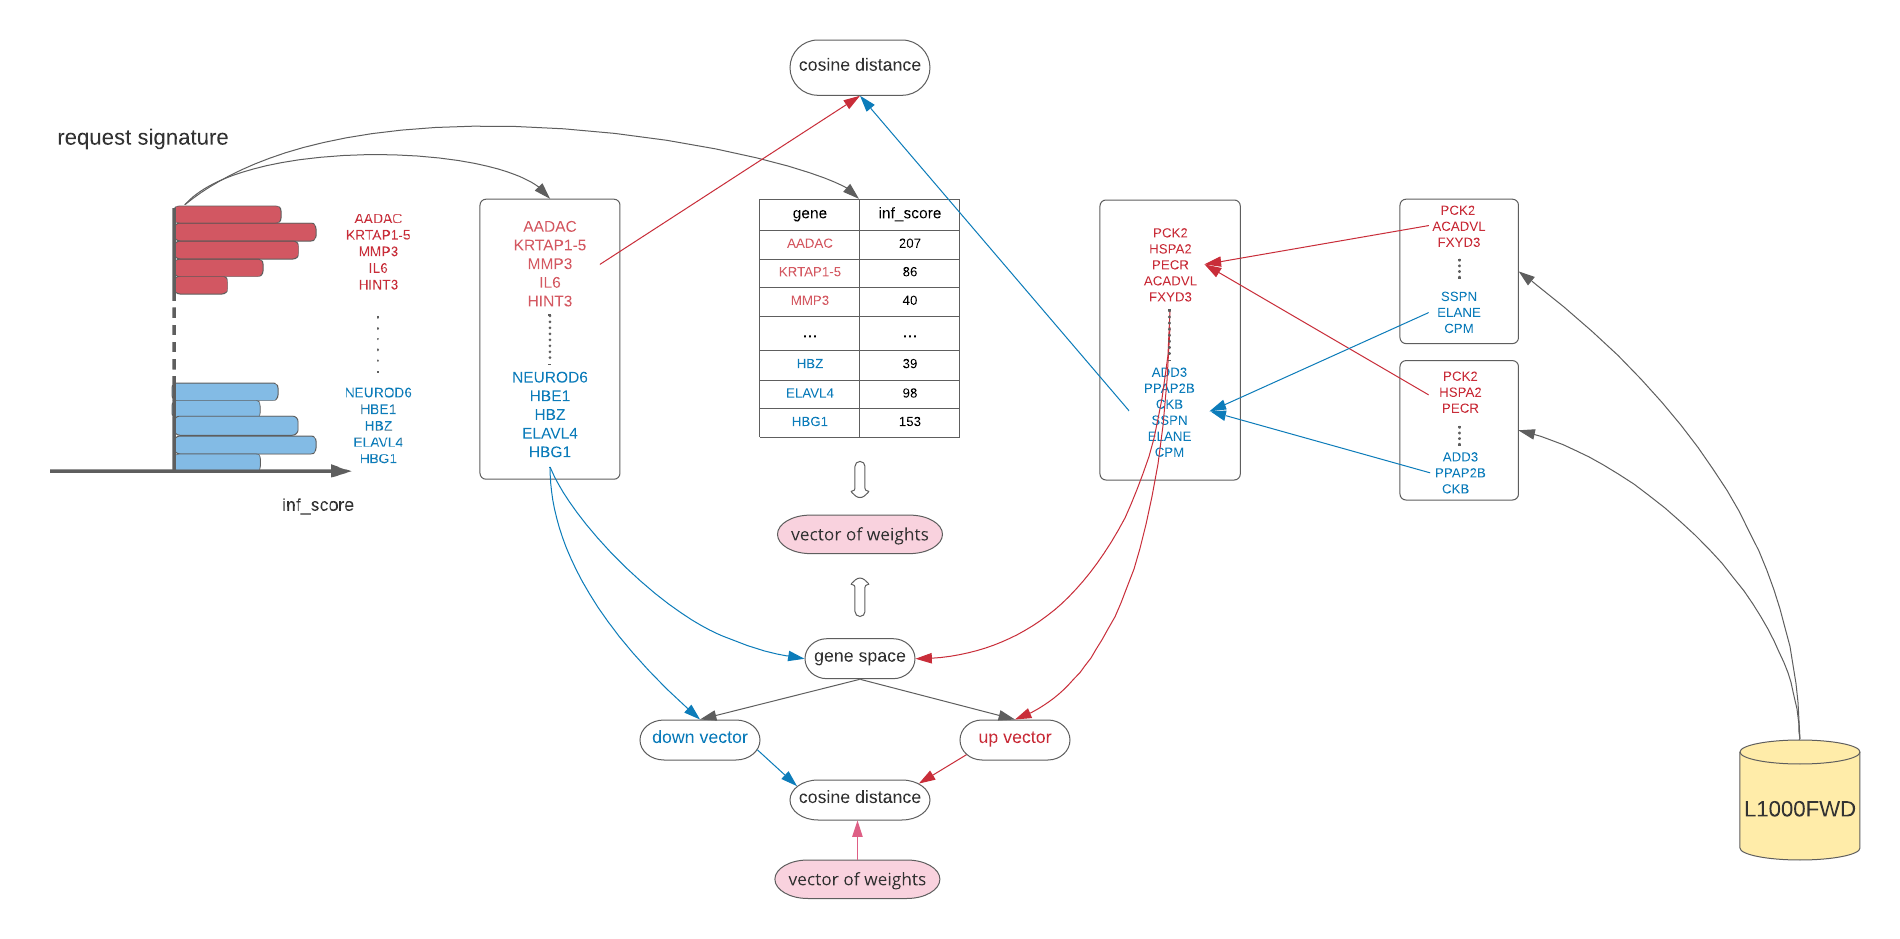
\includegraphics[width=0.8\linewidth]{images/calculating synergy score.png}}
\caption{схема вычисления уровня синергии на основе сравнения сигнатур в "обратном" режиме}
\label{calculating synergy score}
\end{figure}
Для обоих режимов чем  выше уровень синергии, тем больше синергетический эффект.
\subsubsection{Вычисление уровня синергии на основе сравнения обогащенных сигнальных путей}
В этом подходе вместо каждой сигнатуры использовались сигнальные пути, полученные в результате анализа обогащения генов этой сигнатуры с повышенной / пониженной экспрессией. Таким образом каждая сигнатура была представлена 2 списками сигнальных путей: активированные и подавленные. Анализ обогащения проводился с помощью инструмента \href{https://maayanlab.cloud/Enrichr/}{Enrich}  \cite{10.1093/nar/gkw377}.
В данном методе были опробованы 2 способа вычисления уровня синергии на основе сравнения сигнальных путей:
\begin{itemize}
    \item оценка схожести с помощью вычисления коэффициента Танимото
    \item оценка схожести с помощью вычисления взаимной информации
\end{itemize}
\textbf{Вычисление уровня синергии с помощью коэффициента Танимото}


Аналогично предыдущему методу вычисления уровня синергии, для каждой пары сигнатур из базы данных объединялись списки активированных/подавленных сигнальных путей. Таким образом каждая пара сигнатур характеризовалась 2 списками сигнальных путей: активированными и подавленными. 

На следующем этапе оценивалось сходство списков сигнальных путей сигнатуры запроса и сигнатуры пары вычислением коэффициентам Танимото. Коэффициент Танимото измеряет степень схожести двух  множеств и вычисляется по следующей формуле:
\begin{equation}
    Tc=\frac{bc}{b1+b2-bc},
    \label{equation1}
\end{equation}
где b1 - число элементов первого множества, b2 - число элементов второго множества, bc -  количество элементов в пересечении множеств.


В "прямом"\ режиме вычисляется коэффициент Танимото для множества активированных сигнальных путей сигнатуры запроса и множества активированных сигнальных путей сигнатуры пары. Также аналогично вычисляется коэффициент Танимото для множества подавленных сигнальных путей сигнатуры запроса и множества подавленных сигнальных путей сигнатуры пары. В качества оценки уровня синергии берется среднее значение вычисленных коэффициентов Танимото.


В "обратном"\ режиме вычисляется коэффициент Танимото для множества активированных сигнальных путей сигнатуры запроса и множества подавленных сигнальных путей сигнатуры пары. Также аналогично вычисляется коэффициент Танимото для множества подавленных сигнальных путей сигнатуры запроса и множества активированных сигнальных путей сигнатуры пары. В качества оценки уровня синергии берется среднее значение вычисленных коэффициентов Танимото.


На рисунке \ref{enrich_tanimoto} представлена схема вычисления уровня синергии  в "обратном"\ режиме.
\begin{figure}[H]
\center{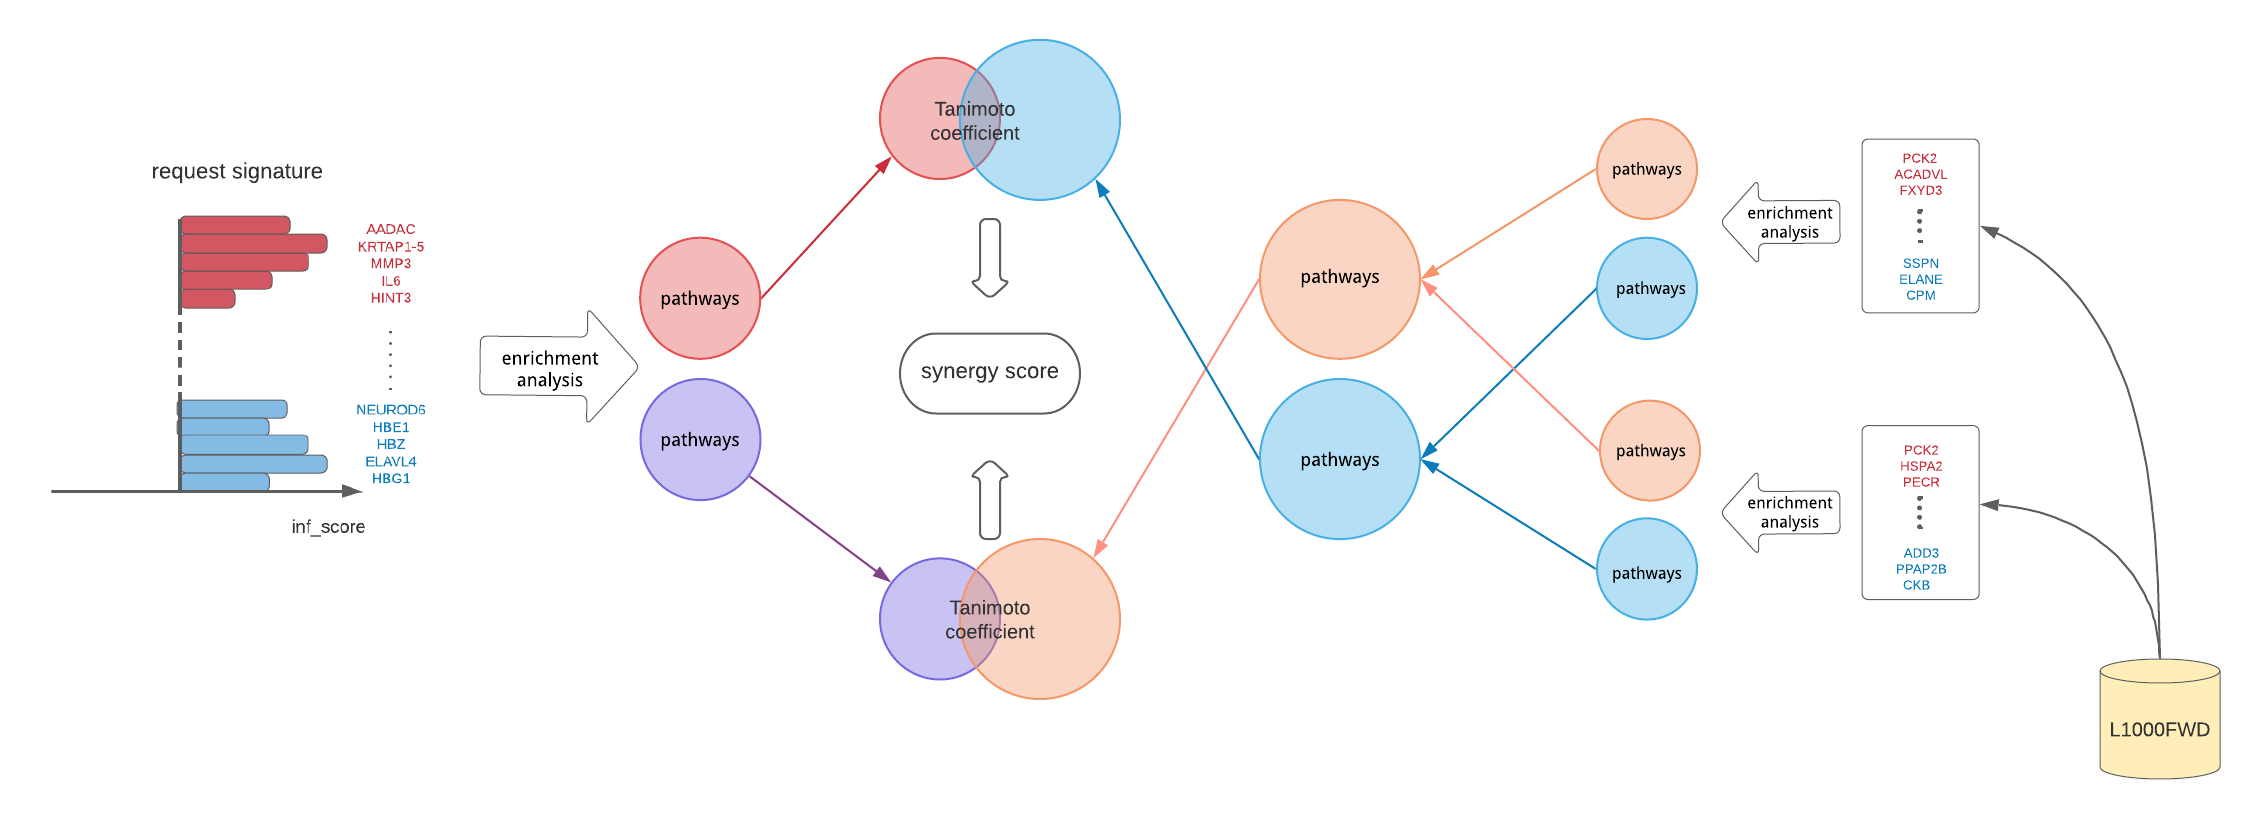
\includegraphics[width=0.8\linewidth]{images/Enrich_Tanimoto_coeff.png}}
\caption{Схема вычисления уровня синергии при использовании коэффициента Танимото в "обратном"\ режиме}
\label{enrich_tanimoto}
\end{figure}

\textbf{Вычисление уровня синергии с помощью взаимной информации}

%Взаимная информация определяется следующим образом:
%\begin{equation}
   % MI={\sum_{i=1}^{|U|}}{\sum_{j=1}^{|V|}}\frac{|U_i \cap V_j|}{N}log{\frac{N|U_i \cap %V_j|}{|U_i||V_j|}}
   % \label{equation1}
%\end{equation}
Взаимная информация также позволяет измерить степень схожести 2 множеств.


В случае "прямого"\ режима сначала для каждой сигнатуры из пары находится пересечение ей соответствующего набора активированных сигнальных путей с набором активированных сигнальных путей сигнатуры запроса. Далее для этих 2 полученных наборов сигнальных путей считается взаимная информация. По аналогии находится пересечение подавленных сигнальных путей сигнатуры из пары и подавленных сигнальных путей сигнатуры запроса. Для этих 2 наборов сигнальных путей также считается взаимная информация. Уровень синергии считается как среднее значение рассчитанных величин взаимной информации. 


В случае "обратного" режима сначала для каждой сигнатуры из пары находится пересечение ей соответствующего набора активированных сигнальных путей с набором подавленных сигнальных путей сигнатуры запроса. Далее для этих 2 полученных  наборов сигнальных путей считается взаимная информация. По аналогии находится пересечение подавленных сигнальных путей сигнатуры из пары и активированных сигнальных путей сигнатуры запроса. Для этих 2 наборов сигнальных путей также считается взаимная информация. Уровень синергии считается как среднее значение рассчитанных величин взаимной информации. 

На рисунке \ref{enrich_MI} представлена схема вычисления уровня синергии в "обратном"\ режиме.
\begin{figure}[H]
\center{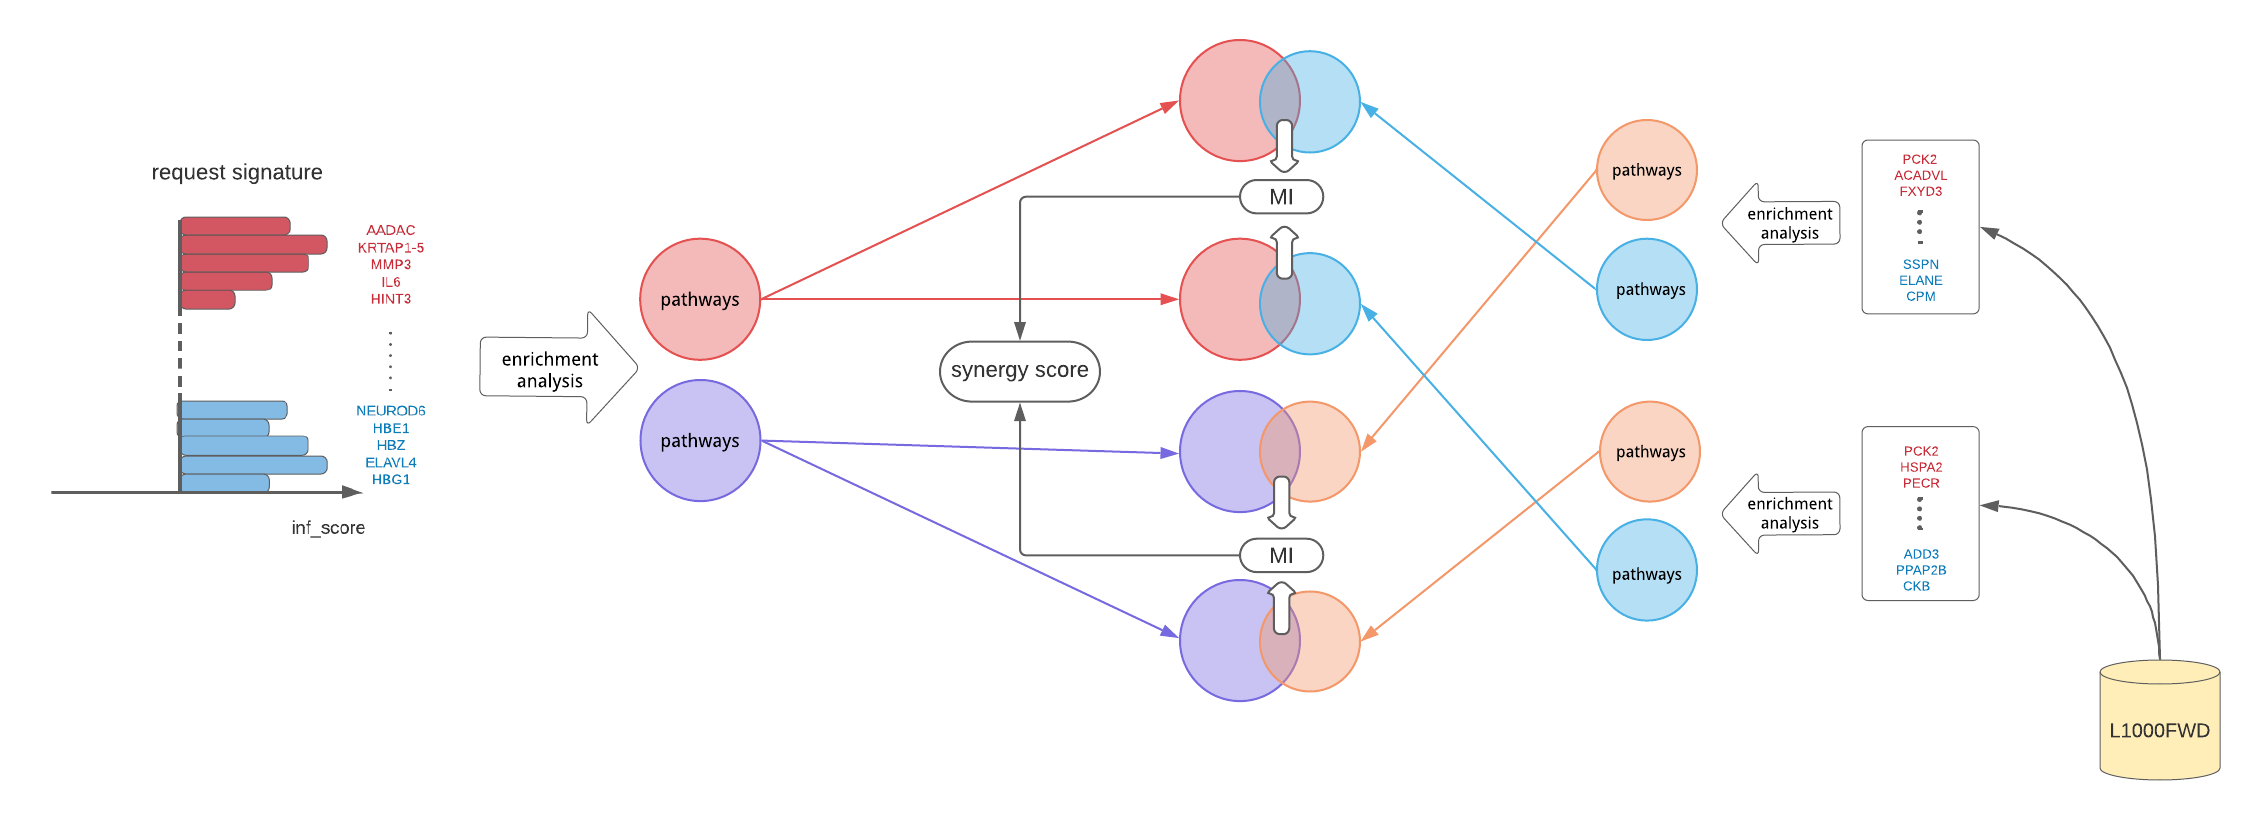
\includegraphics[width=0.8\linewidth]{images/Enrich_MI.png}}
\caption{Схема вычисления уровня синергии при использовании взаимной информации в "обратном"\ режиме}
\label{enrich_MI}
\end{figure}


\subsection{Валидация}
Данный метод разрабатывался в применении к задаче химического перепрограммирования. Для валидации использовалась база данных CFM, которая содержит протоколы химического перепрограммирования клеток. В каждом протоколе приведена синергетическая комбинация малых молекул с указанием исходной и конечной клеточной линии. Также для веществ были дополнительно указаны идентификационные номера (compound identification number, cid) в базе данных \href{https://pubchem.ncbi.nlm.nih.gov/}{PubChem}. 


Для всех малых молекул из базы CFM по их cid были найдены SMILES в базе данных \href{https://pubchem.ncbi.nlm.nih.gov/}{PubChem}. Среди соединений базы L1000FWD есть вещества, которые по химическому строению схожи с малыми молекулами из CFM и, предположительно, обладают схожей активностью. Поэтому при пересечении соединений базы CFM и L1000FWD для последующей валидации было необходимо учесть такие соединения. Для этого для каждого вещества из базы CFM были найдены схожие по строению вещества из базы L1000FWD. Структурное сходство двух молекул оценивалось путем вычисления коэффициента Танимото. В качестве молекулярных отпечатков использовались Morgan Fingerprints. Все пары соединений с коэффициентом  Танимото больше 0.9 считались схожими. При анализе химического сходства использовалась библиотека RDKit \cite{rdkit}.


Для набора малых молекул в каждом протоколе были найдены сигнатуры из L1000FWD, возмущенные этими соединениями. Любую пару малых молекул из одного протокола мы считаем синергетической. Все пары, в которых малые молекулы принадлежат разным протоколам, мы считаем несинергетическими. 


Так как среди рассматриваемых соединений должны быть представлены как синергетические, так и несинергетические пары, мы работали с клеточными переходами, для которых в базе CFM было больше 2 протоколов, и в каждом протоколе было больше 1 молекулы. При работе с конкретным переходом сначала рассчитывалась сигнатура запроса на основе анализа дифференциальной экспрессии между начальным и конечным типом клетки. Использовались данные RNA-seq из базы \href{https://maayanlab.cloud/archs4/data.html}{ARCHS4} \cite{lachmann2018massive} для начального и конечного типа клетки. Затем собирали набор сигнатур по протоколам в CFM для этого перехода. Для каждой пары сигнатур из этого набора был рассчитан уровень синергии. Рассчитанные значения уровня синергии делились на 2 выборки: для синергетических и несинергетических пар. Далее мы сравнивали распределения этих выборок, используя тест Колмогорова-Смирнова, реализованный в библиотеке SciPy. Он используется для проверки гипотезы о принадлежности двух независимых выборок одному закону распределения. Если статистика Колмогорова-Смирнова значима (p<0,05), то эта гипотеза должна быть отвергнута. Нашей задачей было добиться, чтобы метод хорошо разделял синергетические пары от несинергетических по уровню синергии. Соответственно, для нас важными показателями были p-value и разница между средним значением уровня синергии для несинергетических пар и средним значением уровней синергии для синергетических пар. На рисунке \ref{Схема валидации} ниже приведена схема валидации. 
\begin{figure}[H]
\center{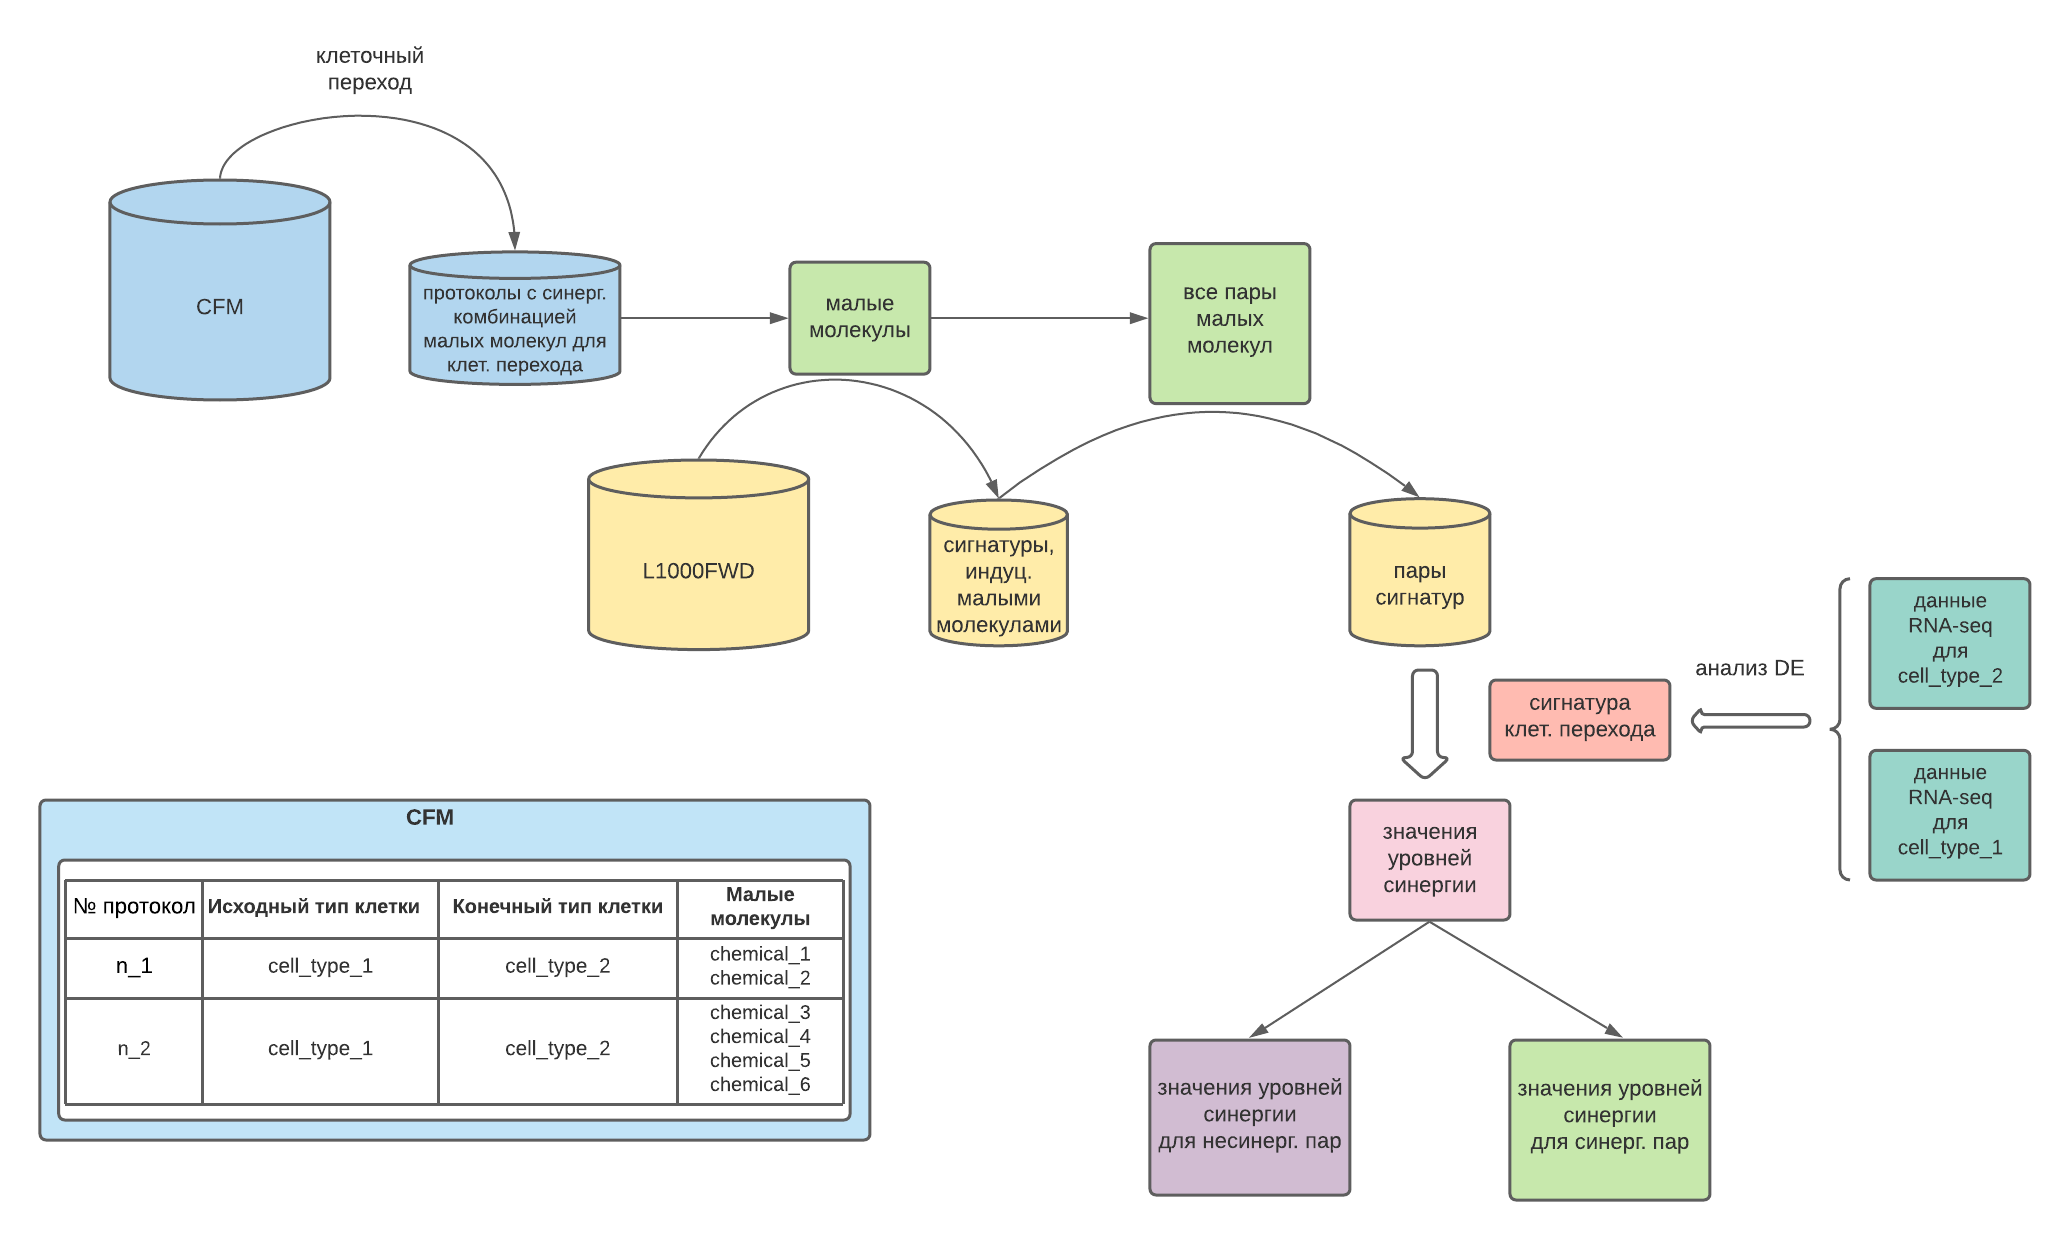
\includegraphics[width=0.9\linewidth]{images/validation.png}}
\caption{Схема валидации}
\label{Схема валидации}
\end{figure}
Нашей задачей было подобрать коэффициенты в выражении inf\_score, при которых метод работал на всех клеточных переходах. При валидации на каждом клеточном переходе на большинстве наборов коэффициентов p-value было достаточно низким, поэтому нас интересовала максимальная разница средних значений уровня синергии для несинергетических пар и синергетических пар. Соответственно разница средних значений уровня синергии для несинергетических пар и синергетических пар рассматривалась как функция коэффициентов. Нашей задачей было найти коэффициенты при максимуме этой функции. Для этого использовали байесовский оптимизатор, поскольку он подходит для задач, где целевая функция неизвестна.
Таким образом, для каждого перехода были найдены оптимальные коэффициенты. Далее коэффициенты в выражении inf\_score были определены как средние значения найденных оптимальных коэффициентов по всем возможным клеточным переходам в базе CFM.
